\textbf{{1. 组播地址介绍}}

因为组播需要一对多的发送,{\textbf{所以组播一定是仅应用于UDP}}。而TCP是一个面向连接的协议,它意味着分别运行于两台主机(由IP地址来确定)内的两个进程(由端口号来确定)之间存在一条连接,所以是一对一的发送。

{\textbf{2. IP组播的思想}}

源主机只发送一份数据,该数据中的{\textbf{目的地址为组播的组地址}}。组地址中的所有接收者都可以接收到同样的数据副本,并且只有组播内的主机可以接收数据,网络中的其他主机不可能收到该数据。\\

与广播所不同的是,\textbf{主机组播时仅发送一份数据,组播的数据仅在传送路径分岔时才将数据报复制后继续转发},单播和组播的传播过程如下图所示。采用组播协议可明显地减轻网络中各种资源的消耗。\textbf{{组播需要路由器的支持才能实现,能够运行组播协议的路由器称为组播路由器}。}

\textbf{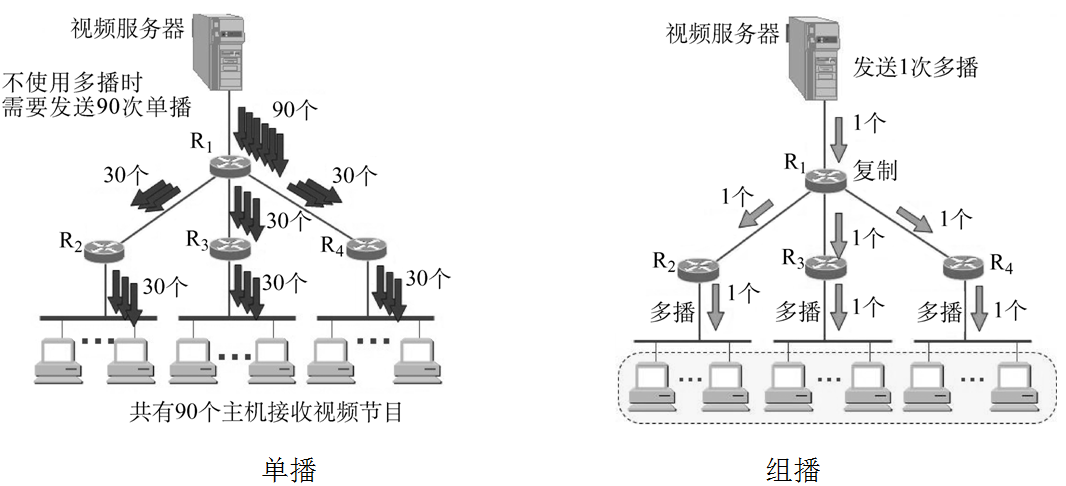
\includegraphics[width=3.33333in,height=1.52083in]{png-jpeg-pics/22E028E75BD2B29A8C79154A3C22AAB7.png}\\
}
